\documentclass[12pt, draftclsnofoot, onecolumn]{IEEEtran}
%\documentclass[]{IEEEtran}
\usepackage{cite}
\usepackage{graphicx}
\usepackage{subcaption}
\usepackage{color}
\usepackage{hyperref}
\graphicspath{{./images/}}


\newcommand{\figref}[1]{Figure~\ref{fig:#1}}


\title{The SR-71 Blackbird}
\author{Nakul Joshi\thanks{
	Nakul Joshi is a senior majoring in Computer Engineering. He enjoys running, reading, and keeping up with developments in science and technology. Contact him at \href{mailto:nakuljos@usc.edu}{nakuljos@usc.edu} or at 213-610-6105.
}}
\begin{document}
\maketitle

\begin{abstract}
	Beautiful and fast, the Lockheed SR-71 ``Blackbird'' was amongst the most successful reconnaissance aircraft ever built. A marvel of engineering, it fulfilled its military role perfectly: not one was lost to enemy action. Retired for political reasons in 1998, it continues to hold the record for fastest manned air-breathing craft. Recently, Lockheed announced the development of the Blackbird's successor, the unmanned SR-72 ``Aurora". This paper examines the various innovations that made possible the unique capabilities of the Blackbird.
\end{abstract}

\begin{IEEEkeywords} lockheed, skunk works, sr, blackbird, aurora \end{IEEEkeywords}



\section{Introduction}

	\IEEEPARstart{T}{he} need for a high-speed stealth reconnaissance aircraft was recognised by the CIA in 1960, after the downing of a U2 aircraft over Soviet airspace. The U2 was thought to be safe from enemy radar at its 20km altitude, but the relatively slow craft was intercepted by Soviet planes near the Ural mountains~\cite{u2}, causing an escalation of tensions during the Cold War. The CIA then commissioned the design and construction of a plane that could fly faster and higher than the U2, while still being able to take high-quality photographs over enemy terrain.	
	
	\subsection*{Description}

	\begin{figure}[h]
		\centering
		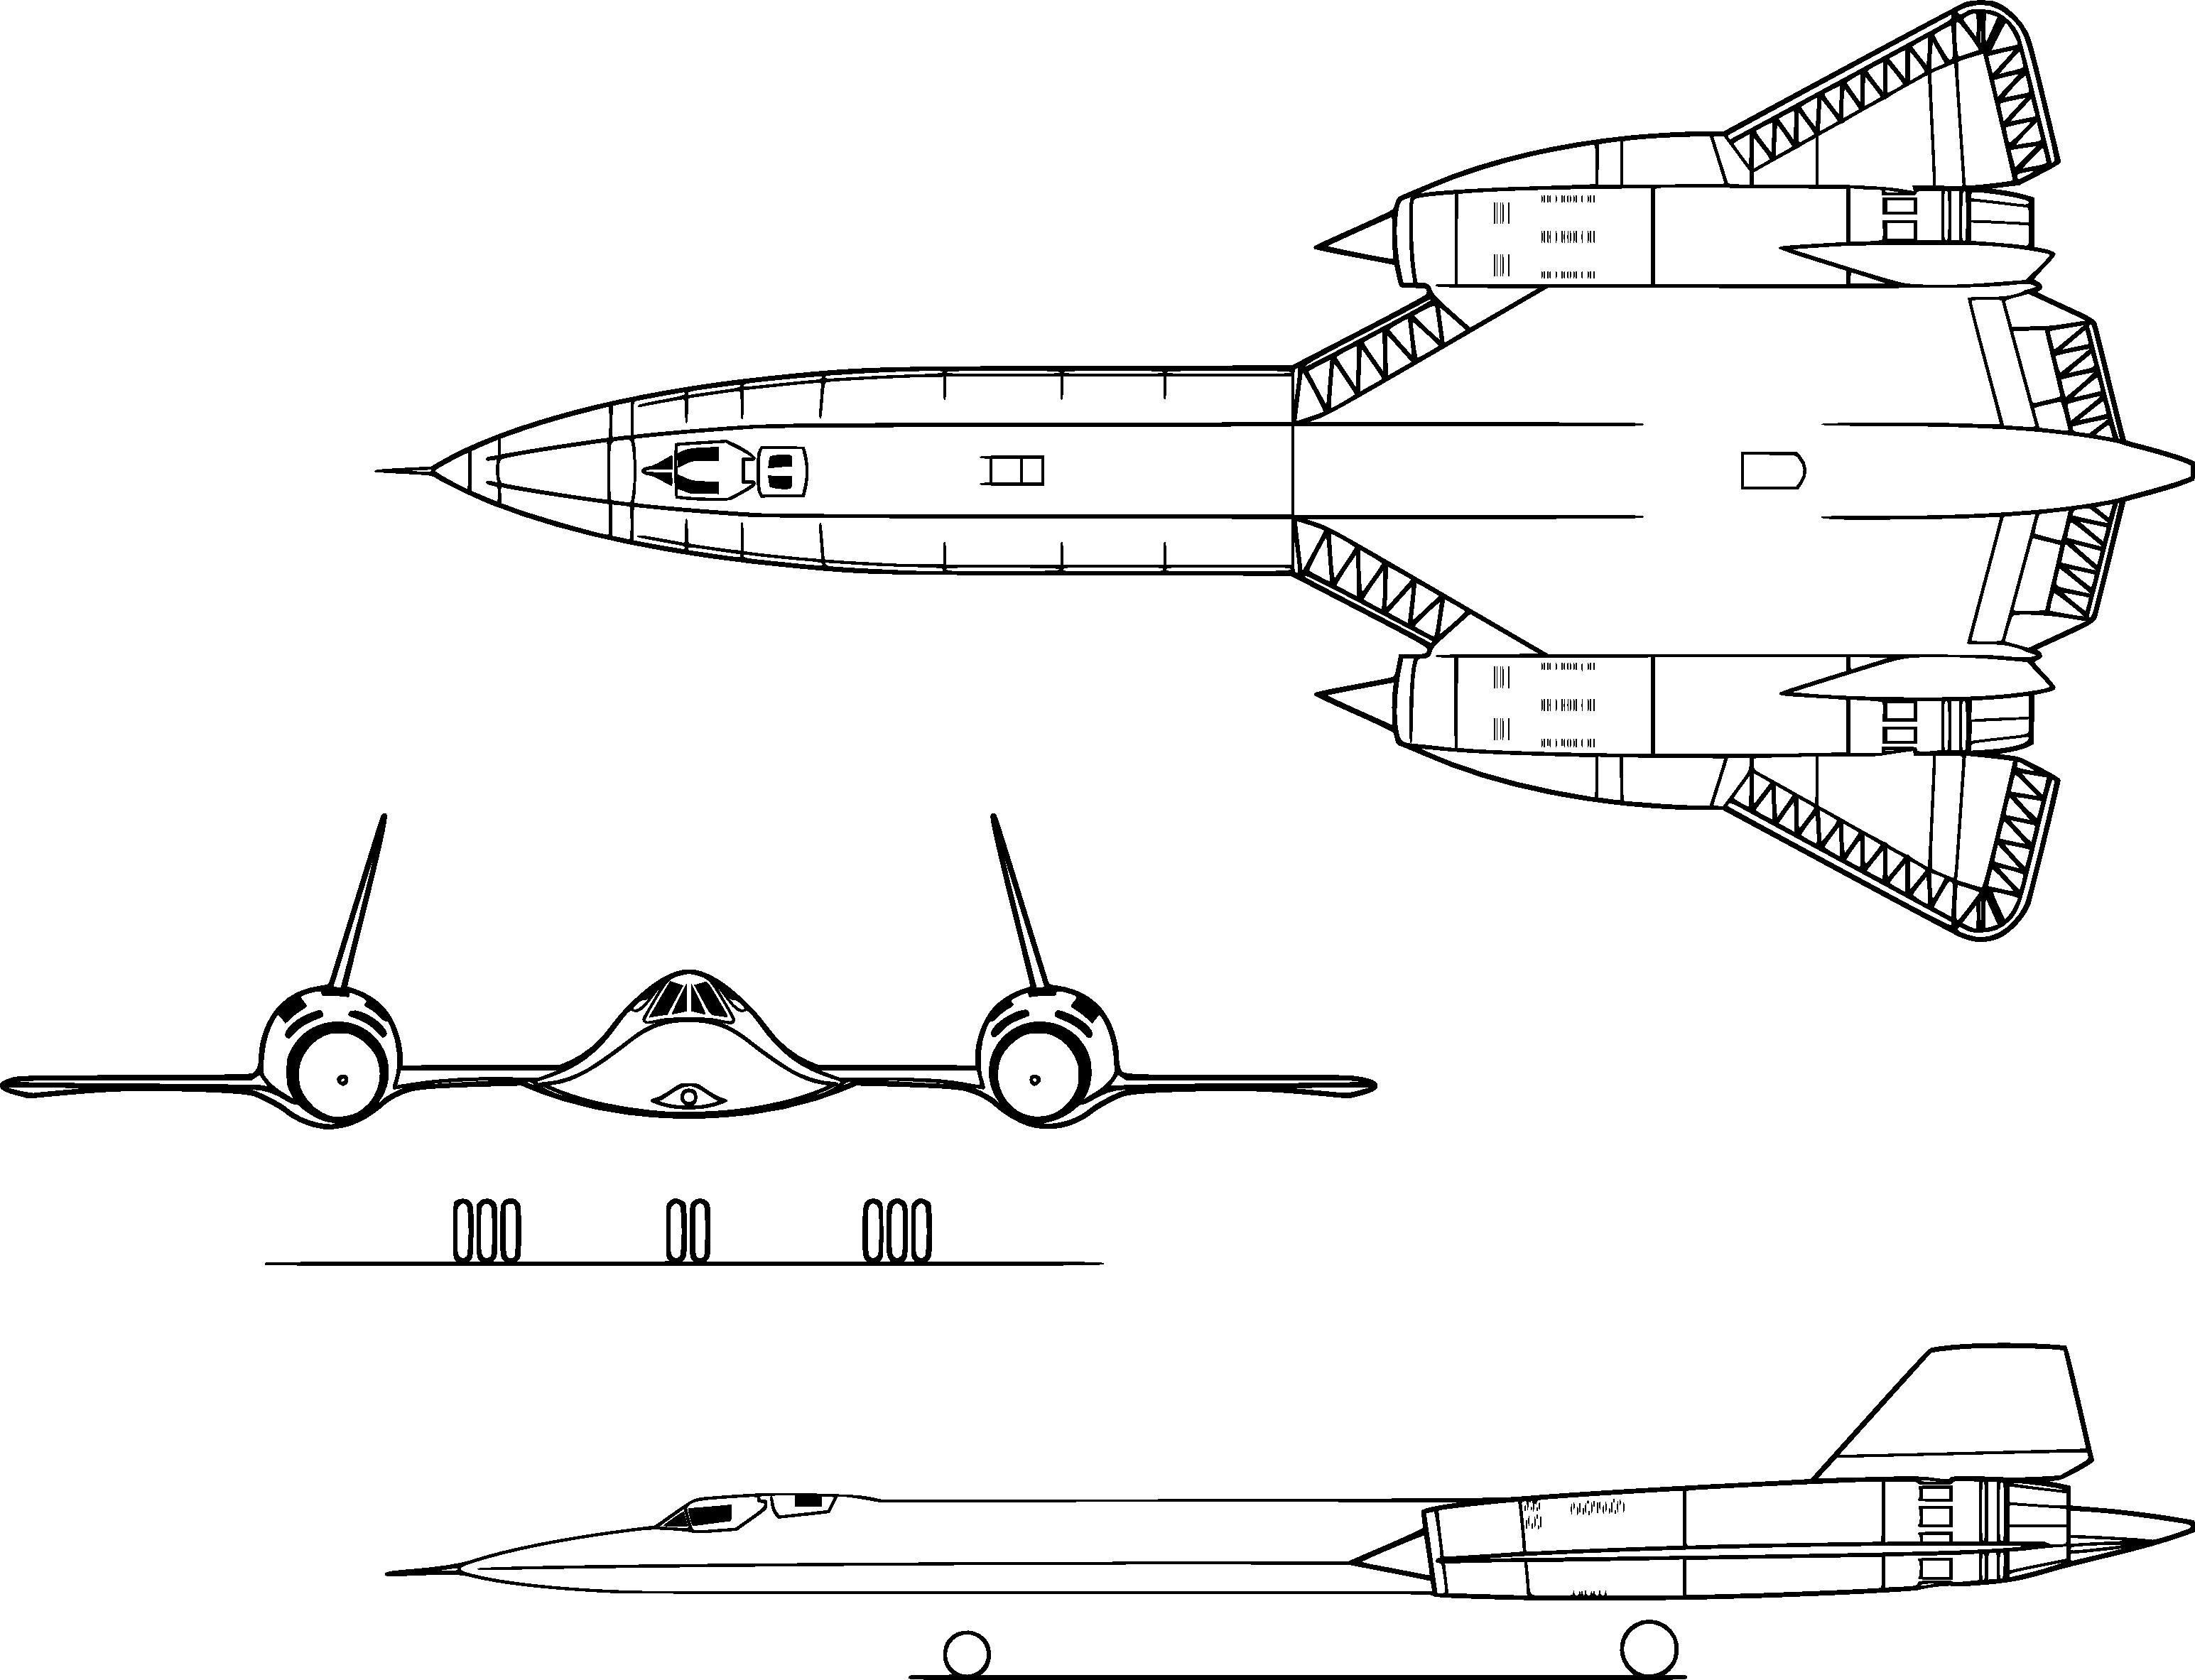
\includegraphics[width=0.8\textwidth]{view.pdf}
		\caption{Views of the SR-71A}
	\end{figure}

	Three versions of the craft were built: the main production variant was designated as SR-71A, while the trainer variant was named the SR-71B. A third variant, built from the remains of a YF-12A craft, was designated SR-71C.
	The unique shape of the craft was specifically designed to minimize radar cross-section (a measure of how detectable it was to radar). It had a length of 32.74 m and a wingspan of 16.94 m. It was capable of flying 5,400 km at up to Mach 3.3 (3,540 km/h), at a cruising altitude of 24,000 m.


	\subsection*{Operational History}
	The contract for the Blackbird was awarded to Skunk Works, a division of Lockheed that had already completed advanced and top secret projects such as the A-12, another high-speed aircraft. Test flights commenced in 1964, while the first SR-71 entered service in 1966. A total of 32 SR-71s were built: 29 SR-71As, 2 SR-71Bs, and the one SR-71C. The craft were used for surveillance over such hostile territories as Vietnam, China, and North Korea. Flights over the Soviet Union had technically been banned since the 1960 U2 incident, but the Blackbird's high cruising altitude allowed it to gather data without entering Soviet airspace. It was extremely successful; none were shot down or otherwise lost to the enemy. By 1990, the Blackbirds had clocked more than 11,000 mission flight hours over some 3,500 missions, spending about 2,750 mission flight hours at Mach 3 speeds\cite{stats}.

	However, the program began to lose support from Air Force officials, who saw it as a chip to trade in for newer programs like the B1-Lancer. The high operating costs of the aircraft made it a target for congressmen too\cite{stats}. Other technologies, like drones and orbital recon, were becoming prominent as well. These factors led to the halting of the SR-71 program in 1989, with six units left in storage and ready to be re-enabled within sixty days if necessary. This allowed the program to be reactivated by Congress in 1993, when political tensions had begun growing in the Middle East as well as North Korea\cite{retirement}. The reactivation was met by resistance from the Air Force, however, and the project was stopped for good in 1998, with two units being given to NASA for a year and the rest being sent to museums around the United States.
	
\begin{figure}[h]
	\centering
	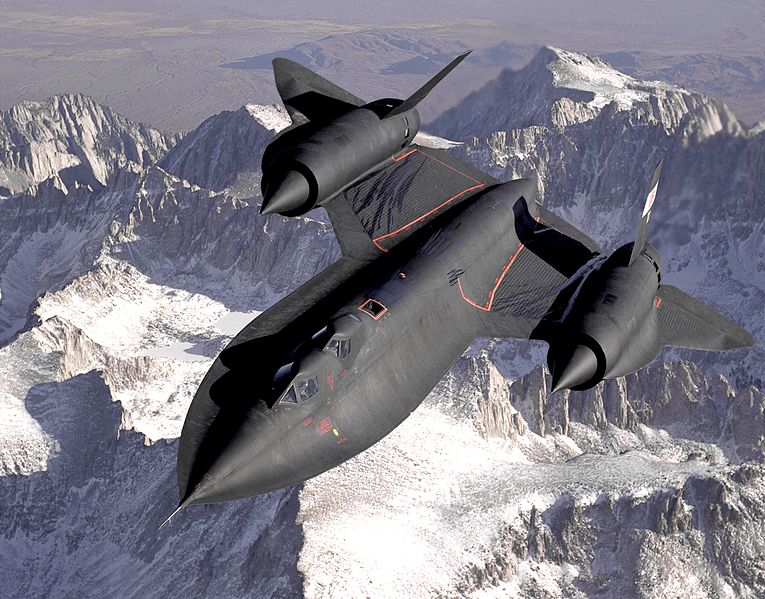
\includegraphics[width=0.8\textwidth]{sr71b.jpg}
	\caption{An SR-71B operated by NASA~\cite{dryden}. Note the instructor's raised cockpit.}
\end{figure}

	
\section{Engineering}

The SR-71 was far ahead of its time. To put just how far into perspective, one only has to observe that its first flight was three years before the introduction of the world's first pocket calculator in 1967. Consequently, it had to be designed by hand, with a slide rule and graph paper. Its cutting-edge performance characteristics stand as a testament to the genius and meticulousness of the engineers at Lockheed. In this section, we discuss some of the innovations that went into the SR-71.

	\subsection*{Engines}
	The Blackbird's engines are perhaps the single most impressive feature of the craft. Its twin Pratt \& Whitney J58-P4 powerplants delivered a total thrust of 300 kilonewtons\cite{engines} to the craft, sufficient to power a small cruise ship. The engines had to be specially configured to counter several issues that were unique to the Blackbird: they had to generate enormous power in the low-oxygen environment of 80,000 feet, all the while contending with the extreme heat generated both by the engines themselves as well as atmospheric resistance.
	
	In a more conventional engine operation, moving air has to be slowed down and compressed to high pressures before it can be used to ignite fuel. This is typically done with a turbojet, whose spinning blades compress the air and forward it to a turbine where it is combusted. To fly faster, the fuel has to be burned at a higher rate, which requires more air to be compressed into the turbine. However, this also makes the fuel burn hotter, meaning that a plane can only fly so fast before its engines melt. A conventional turbojet, with its many small moving parts, cannot withstand the temperatures needed for Mach3 flight.
	
	 Getting around this limit of turbojet capability called for an ingenious hybrid design: the J58 had a turbojet \emph{inside} a non-moving ramjet engine. The turbojet engine operated at subsonic speeds (see \figref{subsonic}), actively sucking in air to ignite fuel.
	 
	\begin{figure}[h]
	\centering
		\begin{subfigure}{0.8\textwidth}
			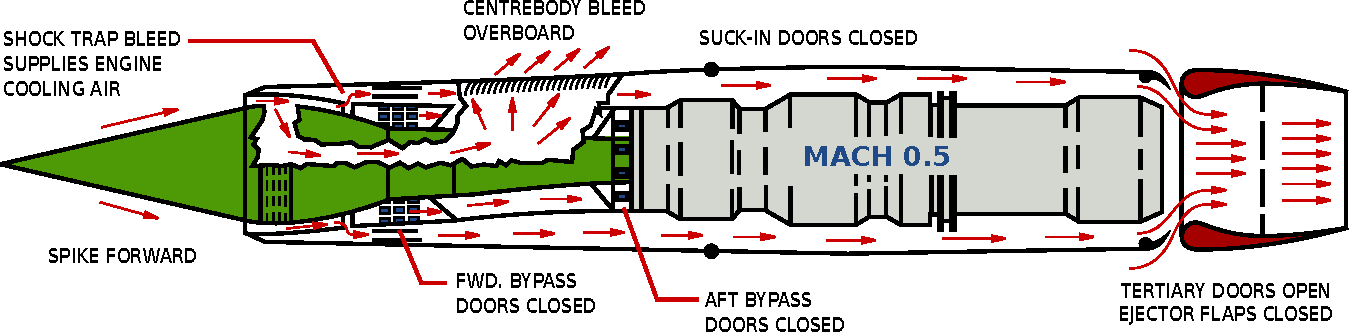
\includegraphics[width=\textwidth]{mach05.pdf}
			\caption{Subsonic operation mode.}\label{fig:subsonic}
		\end{subfigure}
		\begin{subfigure}{0.8\textwidth}
			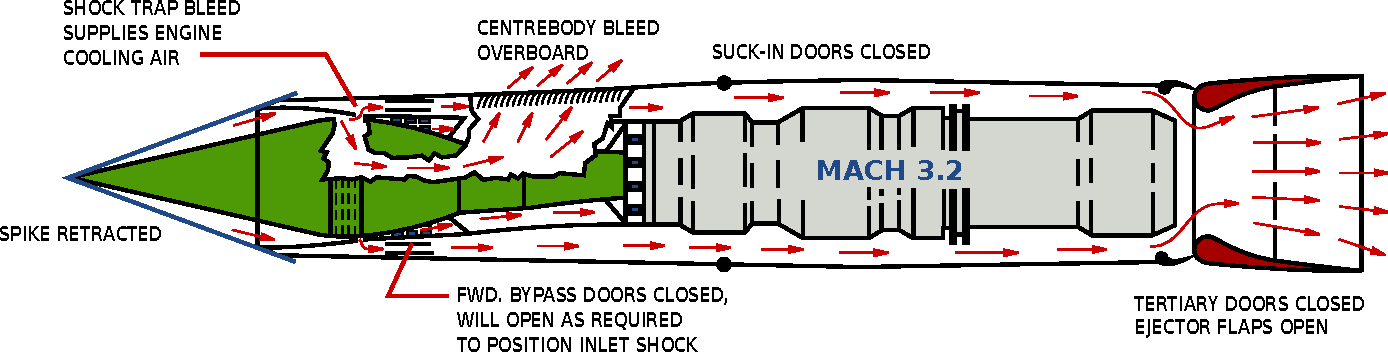
\includegraphics[width=\textwidth]{mach32.pdf}
			\caption{Supersonic operation mode.}\label{fig:supersonic}
		\end{subfigure}
		\caption{Engine airflow diagrams.}
	\end{figure}
	
	As the craft accelerated, the turbojets ceased to operate: at high speeds, air began entering the engines so fast that air had to be kept out rather than sucked in. The forward spikes in front of the engine began retracting, routing air around the turbojet and into the ramjet engine (see \figref{supersonic}). Ramjets need no moving parts, since the speed of the aircraft is itself sufficient to compress the air. This allows them to withstand the high temperatures more easily. One unexpected upshot of this design was that the plane became more fuel-efficient the faster it went, achieving peak efficiency at Mach 3.2. Pilots were limited to this speed for fear of damaging the plane, but former pilot Brian Shul fondly recalls that ``the jet would always give you a little more speed if you wanted it to"\cite{sleddriver}.
	

	\subsection*{Stealth}
	
		As a reconnaisance vehicle, the Blackbird had to evade sight and radar. Some of the incoming radar was absorbed by special materials incorporated into the aircraft's skin, while the rest was deflected by the wings' flattened, tapering design. The mid-wing engine configuration did much to reduce the plane's heat signature. Keeping up with advancing Soviet radar technology was vital, and the government pushed for smaller, stealthier profiles. Radar tests, carefully timed to avoid observation by Soviet satellites, showed that Lockheed had succeeded in building a plane that, on radar, looked only as big as a person~\cite{creating}.
		
		Overall, however, stealth features were difficult to add to such a high powered plane, and so it ultimately had to rely on its high altitude and speed to avoid detection. If spotted, the plane simply accelerated and escaped. The strategy worked because the Blackbird was faster than anything else in the sky; none of the over 4000\cite{sleddriver} missiles fired at it ever managed to catch up.
		
		These characteristics allowed the Blackbird to perform its job with impunity. Only one aircraft came close to matching it, the USSR's MiG-25 ``Foxbat", but it too failed to ever successfully intercept an SR-71. Indeed, Blackbird pilots have reported~\cite{sleddriver} incidents in which Foxbats, after detecting Blackbirds, made futile attempts at chasing them, only to drop out of the sky several minutes later after running out of fuel.
		
	\subsection*{Hull}
		The Blackbird's cruising speed would subject it to shocks and stresses no craft had experienced before. The plane would reach over 300$^\circ$C in flight, so hot that some pilots took to heating up their meals by jamming them against the inner surface of their windscreens~\cite{bbc}. Getting around this issue called for an all-titanium hull, a first in aerospace history.
		
		However, the United States did not have titanium of the grade needed~\cite{skunkworks}. Ironically, the requisite titanium ore was sourced from the Soviet Union, under the cover of shadow companies set up in third world countries by the CIA~\cite{bbc,skunkworks}. More problems emerged when the ore arrived: chlorine in tap water corroded it, and so it had to be treated with distilled water~\cite{skunkworks}. Further, the existing cadmium-plated tooling machinery made it brittle, which meant that new tooling had to be custom-built for the craft, itself all in titanium. The effort paid off, and the hull only strengthened with time as the heat it endured caused it to anneal.
		
		An interesting property of the hull was that its plates had to be kept very loose, to allow slack for thermal expansion under the high temperatures it would experience; consequently, the Blackbird leaked fuel on the runway during takeoff. After takeoff, the Blackbird would run a short sprint to heat the hull and seal the gaps, after which it could refuel in mid-air before proceeding on its mission.

\section{Conclusion}

	The Blackbird was an impressive work of engineering, setting bars that have not been broken more than a decade after its retirement. More a spacecraft than a plane, it was designed beyond the imaginable limits of the time without any of the powerful computing infrastructures that we take for granted today. The Blackbird thus stands as a symbol of what can be achieved when ingenuity meets determination. The technologies that came out of its development are still in use in aircraft today, and it will be interesting to see what new innovations will spill out of its planned successor, the SR-72.
	
\begin{figure}
	\centering
	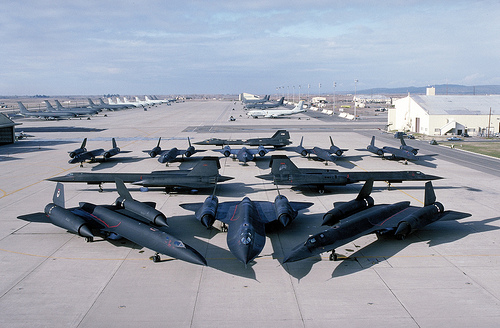
\includegraphics[width=0.7\textwidth]{fleet}
	\caption{Fleet of Blackbirds~\cite{flickr}.}
\end{figure}

\bibliography{citations}{}
\bibliographystyle{plain}
\end{document}
